% Created 2024-10-02 Ср 20:42
% Intended LaTeX compiler: pdflatex
\documentclass[14pt]{extarticle}
\usepackage[utf8]{inputenc}
\usepackage[T2A]{fontenc}
\usepackage{graphicx}
\usepackage{longtable}
\usepackage{wrapfig}
\usepackage{rotating}
\usepackage[normalem]{ulem}
\usepackage{amsmath}
\usepackage{amssymb}
\usepackage{capt-of}
\usepackage{hyperref}
\usepackage[russian]{babel}
\usepackage{tempora}
\usepackage{geometry}
\geometry{a4paper, left=30mm, top=20mm, bottom=20mm, right=15mm }
\usepackage{graphicx}
\usepackage{array}
\usepackage{tabularx}
\usepackage{listings}
\usepackage{float}
\usepackage{setspace}
\usepackage{tabularx}
\usepackage{longtable}
\usepackage{titlesec}
\titleformat{\section}{\normalsize\bfseries}{}{1.25cm}{}
\titleformat{\subsection}{\normalsize\bfseries}{}{1.25cm}{}
\titleformat{\subsubsection}{\normalsize\bfseries}{}{1.25cm}{}
\addto\captionsrussian{\renewcommand{\contentsname}{\centering \normalsize СОДЕРЖАНИЕ}}
\addtocontents{toc}{\protect\thispagestyle{empty}}
\usepackage{titletoc}
\titlecontents{section}[0pt]{}{\contentsmargin{0pt} \thecontentslabel\enspace}{\contentsmargin{0pt}}{\titlerule*[0.5pc]{.}\contentspage}[]
\dottedcontents{subsection}[3.1em]{}{1.5em}{0.5pc}
\usepackage{caption}
\DeclareCaptionLabelSeparator{custom}{ -- }
\captionsetup[figure]{name=Рисунок, labelsep=custom, font={onehalfspacing}, justification=centering}
\usepackage{ragged2e}
\justifying
\setlength\parindent{1.25cm}
\sloppy
\usepackage{indentfirst}
\usepackage{multirow}
\usepackage{lscape}
\renewcommand{\labelitemi}{\textsc{--}}
\linespread{1.3}
% Настройка caption для стиля
\DeclareCaptionStyle{leftalign}{justification=raggedright}
\captionsetup[listing]{style=leftalign, labelsep=custom, name=Листинг} % Правим позицию заголовка для listing
\usepackage{enumitem}
\setlist[enumerate]{itemindent=1.85cm,leftmargin=0pt}
\author{Vasya Pankov}
\date{\today}
\title{ОПРЕДЕЛЕНИЕ ЭЛЕКТРИЧЕСКОГО СОПРОТИВЛЕНИЯ}
\hypersetup{
 pdfauthor={Vasya Pankov},
 pdftitle={ОПРЕДЕЛЕНИЕ ЭЛЕКТРИЧЕСКОГО СОПРОТИВЛЕНИЯ},
 pdfkeywords={},
 pdfsubject={},
 pdfcreator={Emacs 29.4 (Org mode 9.6.15)}, 
 pdflang={Russian}}

% Setup for code blocks [1/2]

\usepackage{fvextra}

\fvset{%
  commandchars=\\\{\},
  highlightcolor=white!95!black!80!blue,
  breaklines=true,
  breaksymbol=\color{white!60!black}\tiny\ensuremath{\hookrightarrow}}

% Make line numbers smaller and grey.
\renewcommand\theFancyVerbLine{\footnotesize\color{black!40!white}\arabic{FancyVerbLine}}

\usepackage{xcolor}

% In case engrave-faces-latex-gen-preamble has not been run.
\providecolor{EfD}{HTML}{f7f7f7}
\providecolor{EFD}{HTML}{28292e}

% Define a Code environment to prettily wrap the fontified code.
\usepackage[breakable,xparse]{tcolorbox}
\DeclareTColorBox[]{Code}{o}%
{colback=EfD!98!EFD, colframe=EfD!95!EFD,
  fontupper=\footnotesize\setlength{\fboxsep}{0pt},
  colupper=EFD,
  IfNoValueTF={#1}%
  {boxsep=2pt, arc=2.5pt, outer arc=2.5pt,
    boxrule=0.5pt, left=2pt}%
  {boxsep=2.5pt, arc=0pt, outer arc=0pt,
    boxrule=0pt, leftrule=1.5pt, left=0.5pt},
  right=2pt, top=1pt, bottom=0.5pt,
  breakable}

% Support listings with captions
\usepackage{float}
\floatstyle{plain}
\newfloat{listing}{htbp}{lst}
\newcommand{\listingsname}{Listing}
\floatname{listing}{\listingsname}
\newcommand{\listoflistingsname}{List of Listings}
\providecommand{\listoflistings}{\listof{listing}{\listoflistingsname}}


% Setup for code blocks [2/2]: syntax highlighting colors

\newcommand\efstrut{\vrule height 2.1ex depth 0.8ex width 0pt}
\definecolor{EFD}{HTML}{4c4f69}
\definecolor{EfD}{HTML}{eff1f5}
\newcommand{\EFD}[1]{\textcolor{EFD}{#1}} % default
\newcommand{\EFvp}[1]{#1} % variable-pitch
\definecolor{EFh}{HTML}{9ca0b0}
\newcommand{\EFh}[1]{\textcolor{EFh}{#1}} % shadow
\definecolor{EFsc}{HTML}{40a02b}
\newcommand{\EFsc}[1]{\textcolor{EFsc}{#1}} % success
\definecolor{EFw}{HTML}{df8e1d}
\newcommand{\EFw}[1]{\textcolor{EFw}{#1}} % warning
\definecolor{EFe}{HTML}{d20f39}
\newcommand{\EFe}[1]{\textcolor{EFe}{#1}} % error
\definecolor{EFl}{HTML}{7287fd}
\newcommand{\EFl}[1]{\textcolor{EFl}{#1}} % link
\definecolor{EFlv}{HTML}{8b008b}
\newcommand{\EFlv}[1]{\textcolor{EFlv}{#1}} % link-visited
\definecolor{Efhi}{HTML}{e3e4e8}
\newcommand{\EFhi}[1]{\colorbox{Efhi}{\efstrut{}#1}} % highlight
\definecolor{EFc}{HTML}{9ca0b0}
\newcommand{\EFc}[1]{\textcolor{EFc}{#1}} % font-lock-comment-face
\definecolor{EFcd}{HTML}{9ca0b0}
\newcommand{\EFcd}[1]{\textcolor{EFcd}{#1}} % font-lock-comment-delimiter-face
\definecolor{EFs}{HTML}{40a02b}
\newcommand{\EFs}[1]{\textcolor{EFs}{#1}} % font-lock-string-face
\definecolor{EFd}{HTML}{9ca0b0}
\newcommand{\EFd}[1]{\textcolor{EFd}{#1}} % font-lock-doc-face
\definecolor{EFm}{HTML}{fe640b}
\newcommand{\EFm}[1]{\textcolor{EFm}{#1}} % font-lock-doc-markup-face
\definecolor{EFk}{HTML}{8839ef}
\newcommand{\EFk}[1]{\textcolor{EFk}{#1}} % font-lock-keyword-face
\definecolor{EFb}{HTML}{d20f39}
\newcommand{\EFb}[1]{\textcolor{EFb}{#1}} % font-lock-builtin-face
\definecolor{EFf}{HTML}{1e66f5}
\newcommand{\EFf}[1]{\textcolor{EFf}{#1}} % font-lock-function-name-face
\newcommand{\EFv}[1]{#1} % font-lock-variable-name-face
\definecolor{EFt}{HTML}{df8e1d}
\newcommand{\EFt}[1]{\textcolor{EFt}{#1}} % font-lock-type-face
\definecolor{EFo}{HTML}{fe640b}
\newcommand{\EFo}[1]{\textcolor{EFo}{#1}} % font-lock-constant-face
\definecolor{EFwr}{HTML}{df8e1d}
\newcommand{\EFwr}[1]{\textcolor{EFwr}{#1}} % font-lock-warning-face
\definecolor{EFnc}{HTML}{04a5e5}
\newcommand{\EFnc}[1]{\textcolor{EFnc}{#1}} % font-lock-negation-char-face
\definecolor{EFpp}{HTML}{df8e1d}
\newcommand{\EFpp}[1]{\textcolor{EFpp}{#1}} % font-lock-preprocessor-face
\definecolor{EFrc}{HTML}{d20f39}
\newcommand{\EFrc}[1]{\textcolor{EFrc}{#1}} % font-lock-regexp-grouping-construct
\definecolor{EFrb}{HTML}{d20f39}
\newcommand{\EFrb}[1]{\textcolor{EFrb}{#1}} % font-lock-regexp-grouping-backslash
\definecolor{EFob}{HTML}{40a02b}
\definecolor{Efob}{HTML}{e6e9ef}
\newcommand{\EFob}[1]{\colorbox{Efob}{\efstrut{}\textcolor{EFob}{#1}}} % org-block
\definecolor{EFobb}{HTML}{9ca0b0}
\definecolor{Efobb}{HTML}{e6e9ef}
\newcommand{\EFobb}[1]{\colorbox{Efobb}{\efstrut{}\textcolor{EFobb}{#1}}} % org-block-begin-line
\definecolor{EFobe}{HTML}{9ca0b0}
\definecolor{Efobe}{HTML}{e6e9ef}
\newcommand{\EFobe}[1]{\colorbox{Efobe}{\efstrut{}\textcolor{EFobe}{#1}}} % org-block-end-line
\definecolor{EFOa}{HTML}{1e66f5}
\newcommand{\EFOa}[1]{\textcolor{EFOa}{#1}} % outline-1
\definecolor{EFOb}{HTML}{1e66f5}
\newcommand{\EFOb}[1]{\textcolor{EFOb}{#1}} % outline-2
\definecolor{EFOc}{HTML}{1e66f5}
\newcommand{\EFOc}[1]{\textcolor{EFOc}{#1}} % outline-3
\definecolor{EFOd}{HTML}{1e66f5}
\newcommand{\EFOd}[1]{\textcolor{EFOd}{#1}} % outline-4
\definecolor{EFOe}{HTML}{1e66f5}
\newcommand{\EFOe}[1]{\textcolor{EFOe}{#1}} % outline-5
\definecolor{EFOf}{HTML}{1e66f5}
\newcommand{\EFOf}[1]{\textcolor{EFOf}{#1}} % outline-6
\definecolor{EFOg}{HTML}{d20f39}
\newcommand{\EFOg}[1]{\textcolor{EFOg}{#1}} % outline-7
\definecolor{EFOh}{HTML}{40a02b}
\newcommand{\EFOh}[1]{\textcolor{EFOh}{#1}} % outline-8
\newcommand{\EFhn}[1]{#1} % highlight-numbers-number
\newcommand{\EFhq}[1]{#1} % highlight-quoted-quote
\newcommand{\EFhs}[1]{#1} % highlight-quoted-symbol
\newcommand{\EFrda}[1]{#1} % rainbow-delimiters-depth-1-face
\newcommand{\EFrdb}[1]{#1} % rainbow-delimiters-depth-2-face
\newcommand{\EFrdc}[1]{#1} % rainbow-delimiters-depth-3-face
\newcommand{\EFrdd}[1]{#1} % rainbow-delimiters-depth-4-face
\newcommand{\EFrde}[1]{#1} % rainbow-delimiters-depth-5-face
\newcommand{\EFrdf}[1]{#1} % rainbow-delimiters-depth-6-face
\newcommand{\EFrdg}[1]{#1} % rainbow-delimiters-depth-7-face
\newcommand{\EFrdh}[1]{#1} % rainbow-delimiters-depth-8-face
\newcommand{\EFrdi}[1]{#1} % rainbow-delimiters-depth-9-face
\definecolor{EFany}{HTML}{df8e1d}
\newcommand{\EFany}[1]{\textcolor{EFany}{#1}} % ansi-color-yellow
\definecolor{EFanr}{HTML}{d20f39}
\newcommand{\EFanr}[1]{\textcolor{EFanr}{#1}} % ansi-color-red
\definecolor{EFanb}{HTML}{bcc0cc}
\newcommand{\EFanb}[1]{\textcolor{EFanb}{#1}} % ansi-color-black
\definecolor{EFang}{HTML}{40a02b}
\newcommand{\EFang}[1]{\textcolor{EFang}{#1}} % ansi-color-green
\definecolor{EFanB}{HTML}{1e66f5}
\newcommand{\EFanB}[1]{\textcolor{EFanB}{#1}} % ansi-color-blue
\definecolor{EFanc}{HTML}{179299}
\newcommand{\EFanc}[1]{\textcolor{EFanc}{#1}} % ansi-color-cyan
\definecolor{EFanw}{HTML}{5c5f77}
\newcommand{\EFanw}[1]{\textcolor{EFanw}{#1}} % ansi-color-white
\definecolor{EFanm}{HTML}{ea76cb}
\newcommand{\EFanm}[1]{\textcolor{EFanm}{#1}} % ansi-color-magenta
\definecolor{EFANy}{HTML}{df8e1d}
\newcommand{\EFANy}[1]{\textcolor{EFANy}{#1}} % ansi-color-bright-yellow
\definecolor{EFANr}{HTML}{d20f39}
\newcommand{\EFANr}[1]{\textcolor{EFANr}{#1}} % ansi-color-bright-red
\definecolor{EFANb}{HTML}{acb0be}
\newcommand{\EFANb}[1]{\textcolor{EFANb}{#1}} % ansi-color-bright-black
\definecolor{EFANg}{HTML}{40a02b}
\newcommand{\EFANg}[1]{\textcolor{EFANg}{#1}} % ansi-color-bright-green
\definecolor{EFANB}{HTML}{1e66f5}
\newcommand{\EFANB}[1]{\textcolor{EFANB}{#1}} % ansi-color-bright-blue
\definecolor{EFANc}{HTML}{179299}
\newcommand{\EFANc}[1]{\textcolor{EFANc}{#1}} % ansi-color-bright-cyan
\definecolor{EFANw}{HTML}{6c6f85}
\newcommand{\EFANw}[1]{\textcolor{EFANw}{#1}} % ansi-color-bright-white
\definecolor{EFANm}{HTML}{ea76cb}
\newcommand{\EFANm}[1]{\textcolor{EFANm}{#1}} % ansi-color-bright-magenta
\begin{document}

\begin{small}
\begin{titlepage}

\linespread{1}\selectfont\centering{ГУАП}

\vspace{32pt}

\centering{КАФЕДРА №1}

\vspace{60pt}

\raggedright{ОТЧЕТ \\
ЗАЩИЩЕН С ОЦЕНКОЙ}
\vspace{14pt}

\raggedright{ПРЕПОДАВАТЕЛЬ}

\vspace{12pt}

\begin{tabularx}{\textwidth}{ >{\centering\arraybackslash}X >{\centering\arraybackslash}X >{\centering\arraybackslash}X }
	 старший преподаватель & &  \\ 
	 \hrulefill & \hrulefill & \hrulefill \\ 
\footnotesize{должность, уч. степень, звание} & \footnotesize{подпись, дата} & \footnotesize{инициалы, фамилия} \\ 
\end{tabularx} 
 
\vspace{48pt} 

\centering{ОТЧЕТ О ЛАБОРАТОРНОЙ РАБОТЕ} 

\vspace{40pt} 

\centering{ОПРЕДЕЛЕНИЕ ЭЛЕКТРИЧЕСКОГО СОПРОТИВЛЕНИЯ} 

\vspace{40pt} 

\centering{По курсу: } 

\vspace*{\fill} 

\raggedright{РАБОТУ ВЫПОЛНИЛ} 

\vspace{10pt} 

\begin{tabularx}{\textwidth}{>{\raggedright\arraybackslash}X  >{\centering\arraybackslash}X >{\centering\arraybackslash}X >{\centering\arraybackslash}X }
СТУДЕНТ ГР. № & М412 & & Vasya Pankov \\ 
	 & \hrulefill & \hrulefill & \hrulefill \\ 
	 &  & \footnotesize{подпись, дата} & \footnotesize{инициалы, фамилия} \\ 
\end{tabularx} 
 
\vspace*{\fill} 

\centering{Санкт-Петербург \the\year} 

\end{titlepage}
\end{small}

\tableofcontents \clearpage


\section{Цель работы}
\label{sec:org79ca03a}

\begin{itemize}
\item Ознакомление с методикой обработки результатов измерений;
определение электрического сопротивления;
\item экспериментальная проверка закона Ома;
\item определение удельного сопротивления нихрома.
\end{itemize}

\section{Описание лабораторной установки}
\label{sec:org2fb4a39}

На рисунке \ref{fig:org949745b} представлены схемы в которых проводились измерения в ходе
лабораторной работы.

\begin{figure}[H]
\centering
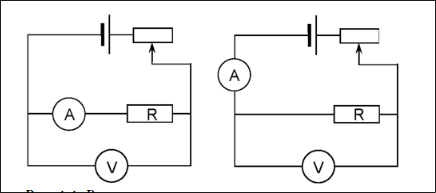
\includegraphics[width=.9\linewidth]{./images/twoSchemes.png}
\caption{\label{fig:org949745b}Использованные измерительные схемы. Слева – схема A, справа – схема B}
\end{figure}

Параметры установки представлены в таблице \ref{tab:org0eccdb8}.

\begin{longtable}{|p{3.9cm}|l|p{2cm}|p{1.3cm}|p{1.2cm}|p{3.6cm}|p{1.2cm}|}
\caption{\label{tab:org0eccdb8}Параметры установки}
\\[0pt]
\hline
Прибор & Тип & Предел измерений & Цена деления & Класс точности & Систематическая погрешность & R, Ом\\[0pt]
\hline
\endfirsthead
\multicolumn{7}{l}{Продолжение с предыдущей страницы} \\[0pt]
\hline

Прибор & Тип & Предел измерений & Цена деления & Класс точности & Систематическая погрешность & R, Ом \\[0pt]

\hline
\endhead
\hline\multicolumn{7}{r}{Продолжение на следующей странице} \\
\endfoot
\endlastfoot
\hline
Вольтметр & МК-2 & 1.5 В & 0.05 & 1.5 & 0.023 В & 2500\\[0pt]
\hline
Миллиамперметр & МК-2 & 250 мА & 5 мА & 1.5 & 3.75 мА & 0.2\\[0pt]
\hline
Линейка & --- & 51 см & 1 мм & --- & 0.5 мм & ---\\[0pt]
\hline
\end{longtable}

\section{Рабочие формулы}
\label{sec:org8b91a45}

Формулы для вычисления электрического сопротивления:

\begin{itemize}
\item закон Ома, формула (\ref{eq:org6db2998});
\item для схемы А, формула (\ref{eq:orgd2e2128});
\item для схемы B, формула (\ref{eq:org957389b}).
\end{itemize}

\begin{equation}
\label{eq:org6db2998}
R = \frac{U}{I}
\end{equation}

\begin{equation}
\label{eq:orgd2e2128}
R = \frac{U}{I} - R_a
\end{equation}

\begin{equation}
\label{eq:org957389b}
R = (\frac{I}{U} - \frac{1}{R_V})^-1
\end{equation}

Используемые обозначения:

\(R\) -- электрическое сопротивление проводника

\(I\) - сила тока в проводнике

\(U\) -- падение напряжения на проводнике

\(R_A\) -- сопротивление амперметра 

\(R_V\) -- сопротивление вольтметра

Для вычисления среднего сопротивления будет использоваться простая
формула среднего арифметического всех имеющихся сопротивлений
представленная в формуле (\ref{eq:orgc7790c1}), где \(n\) - число измерений.


\begin{equation}
\label{eq:orgc7790c1}
R_{avg} = \frac{\sum\limits_{i = 1}^{n} R_i}{n}
\end{equation}

Для вычисления же удельного сопротивления будет использована формула (\ref{eq:org575e93b}),
где используются следующие обозначения:

\begin{itemize}
\item \(\rho\) -- удельное сопротивление
\item \(l\) -- длина провода
\item \(D\) -- диаметр провода
\end{itemize}

\begin{equation}
\label{eq:org575e93b}
\rho = \frac{R_{avg} \pi D^2}{4l}
\end{equation}

\section{Результаты измерений и вычисления}
\label{sec:orga250695}

Результаты измерений и вычислений для схемы А представлены в таблице \ref{tab:org9f22654}.

\begin{longtable}{|l|r|r|r|r|r|r|r|r|r|r|}
\caption{\label{tab:org9f22654}Схема А}
\\[0pt]
\hline
U,В & 0.35 & 0.45 & 0.55 & 0.65 & 0.75 & 0.85 & 0.95 & 1.05 & 1.15 & 1.25\\[0pt]
\hline
\endfirsthead
\multicolumn{11}{l}{Продолжение с предыдущей страницы} \\[0pt]
\hline

U,В & 0.35 & 0.45 & 0.55 & 0.65 & 0.75 & 0.85 & 0.95 & 1.05 & 1.15 & 1.25 \\[0pt]

\hline
\endhead
\hline\multicolumn{11}{r}{Продолжение на следующей странице} \\
\endfoot
\endlastfoot
\hline
I,А & 0.06 & 0.08 & 0.1 & 0.12 & 0.14 & 0.16 & 0.18 & 0.2 & 0.22 & 0.24\\[0pt]
\hline
U/I, Ом & 5.83 & 5.63 & 5.5 & 5.42 & 5.36 & 5.31 & 5.28 & 5.25 & 5.23 & 5.21\\[0pt]
\hline
R, Ом & 5.63 & 5.43 & 5.3 & 5.22 & 5.16 & 5.11 & 5.07 & 5.05 & 5.03 & 5.01\\[0pt]
\hline
\(\Theta_R\), Ом & 0.75 & 0.55 & 0.43 & 0.36 & 0.31 & 0.27 & 0.24 & 0.21 & 0.19 & 0.18\\[0pt]
\hline
\end{longtable}

Результаты измерений и вычислений для схемы B представлены в таблице \ref{tab:org7a4a391}.


\begin{longtable}{|l|r|r|r|r|r|r|r|r|r|r|}
\caption{\label{tab:org7a4a391}Схема B}
\\[0pt]
\hline
U,В & 0.3 & 0.4 & 0.5 & 0.6 & 0.7 & 0.8 & 0.9 & 1.0 & 1.1 & 1.2\\[0pt]
\hline
\endfirsthead
\multicolumn{11}{l}{Продолжение с предыдущей страницы} \\[0pt]
\hline

U,В & 0.3 & 0.4 & 0.5 & 0.6 & 0.7 & 0.8 & 0.9 & 1.0 & 1.1 & 1.2 \\[0pt]

\hline
\endhead
\hline\multicolumn{11}{r}{Продолжение на следующей странице} \\
\endfoot
\endlastfoot
\hline
I,А & 0.06 & 0.08 & 0.1 & 0.12 & 0.14 & 0.16 & 0.18 & 0.2 & 0.22 & 0.24\\[0pt]
\hline
U/I, Ом & 5 & 5 & 5 & 5 & 5 & 5 & 5 & 5 & 5 & 5\\[0pt]
\hline
R, Ом & 5.01 & 5.01 & 5.01 & 5.01 & 5.01 & 5.01 & 5.01 & 5.01 & 5.01 & 5.01\\[0pt]
\hline
\(\Theta_R\), Ом & 0.71 & 0.54 & 0.43 & 0.36 & 0.31 & 0.27 & 0.24 & 0.22 & 0.20 & 0.18\\[0pt]
\hline
\end{longtable}

\(R_avg = 5.1 Om\); \$\(\rho\) = 9.32 \(\cdot\) 10\textsuperscript{-7} Om \(\cdot\) m \$


\section{Примеры вычислений}
\label{sec:orgd89b211}

По формуле (\ref{eq:org6db2998}) \(R = \frac{U}{I} = \frac{0.35}{0.06} \approx 5.83\)

По формуле (\ref{eq:orgd2e2128}) \(R = \frac{U}{I} - R_a = \frac{0.45}{0.08} - 0.2 = 5.625 - 0.2 = 5.425 \approx = 5.43\)

По формуле (\ref{eq:org957389b}) \(R = (\frac{I}{U} - \frac{1}{R_V})^-1 = (\frac{0.06}{3} - \frac{1}{2000})^-1  = (0.2 - 0.0005)^-1 = \frac{1/0.1995} \approx = 5.01\)

По формуле (\ref{eq:orgc7790c1}) \(R = (5.63+5.42+5.3+5.22+5.16+5.11+5.07 + + 5.05+5.03+5.01+5+5+5+5+5+5+5+5+5+5) : 20 = \frac{102}{20} = 5.1\)

По формуле (\ref{eq:org575e93b}) \(\rho = \frac{R_{avg} \pi D^2}{4l} = \frac{5.1 \cdot 3.14 \cdot (0.00032)^2}{4 \cdot 0.44} \approx \frac{1.64 \cdot 10^{-6}}{1.76} \approx 0.931 \cdot \frac{1.64 * 10^{-6}}{1.76}\)


\section{Вычисление погрешности}
\label{sec:org918c2d1}

\subsection{Систематические погрешности}
\label{sec:org03ecdab}

Систематическая погрешность силы тока: \(\Theta_I = \frac{I_m K_I}{100} = \frac{0.25 \cdot 1.5}{100} = 3.75 mA = 0.00375 A\)

Систематическая погрешность напряжения: \(\Theta_U = \frac{U_m K_I}{100} = \frac{1.5 \cdot 1.5}{100} = 0.0225 B\)

Систематическая ошибка вычисления диаметра: \(\Theta_l = 2 \cdot 10^{-3}\) м

Систематическая ошибка линейки: \(\Theta_D = 0.5 \cdot 10^{-5}\) м

Формула (\ref{eq:org7fa976d}) для вычисления систематической погрешности косвенного измерения электрического
сопротивления.

\begin{equation}
\label{eq:org7fa976d}
R = R(U, I) = \frac{U}{I} \\
\Delta
\end{equation}
\end{document}
